\documentclass[11pt,a4paper]{article}
\usepackage[utf8]{inputenc}
\usepackage[T1]{fontenc}
\usepackage{lmodern}
\usepackage{microtype}
\usepackage{geometry}
\geometry{left=2.5cm,right=2.5cm,top=2.6cm,bottom=2.6cm}
\usepackage{amsmath,amssymb}
\usepackage{booktabs,tabularx}
\usepackage{graphicx}
\usepackage{float}
\usepackage{hyperref}
\usepackage{xcolor}
\hypersetup{colorlinks=true,linkcolor=blue!60!black,urlcolor=blue!60!black}
\newcommand{\code}[1]{\texttt{#1}}
\newcommand{\pathcode}[1]{\texttt{\small #1}}
\title{BOAMP Successor Linkage Methodology\\\large Current Benchmark State}
\author{BOAMP Data Science Internship Project}
\date{2026-08-13T21:25:33}
\begin{document}
\sloppy
\maketitle

\section*{Technical Summary}
This report states the current defensible BOAMP successor-linkage pipeline. The
study does not claim to certify legal contract renewals. Its
event is an \emph{observable successor procurement}: a later BOAMP procurement
episode from the same buyer that is sufficiently similar to an earlier awarded
digital procurement episode.

The current Grand Ouest survival cohort contains
3,800 awarded digital procurement episodes.
The main linkage rule accepts 544
successor links, giving an observed event rate of
0.143 and a median observed successor
time of 31.82
months among linked events. The candidate pool is broad:
763,417 candidate pairs from
3,520 anchors with at least one candidate.

The current national benchmark contains 252 labelled anchors
and 7,031 labelled anchor-candidate rows. On the validation split,
\code{M\_B\_text\_ranking @ 0.70} remains the strongest precision-first
choice: precision 0.800, recall 0.182, false-positive
rate 0.000, and 5 accepted validation links.
\code{M\_C\_weighted\_gated} recovers more positives
(recall 0.409) but admits more false positives
(FPR 0.105). This trade-off is important because a false positive in a
survival dataset creates both a false event and a false event time, while an
abstained link is handled conservatively as right-censoring.

\section{What The Pipeline Measures}
Let \(i\) index an earlier awarded procurement episode and \(j\) index a later
candidate episode. The object of interest is not a legal renewal certificate,
because BOAMP notices do not provide that ground truth consistently. Instead,
the pipeline estimates whether the data show a later procurement episode that is
credible enough to be treated as a successor:
\[
Y_i =
\begin{cases}
1, & \text{if one accepted observable successor is found before the cutoff,}\\
0, & \text{otherwise.}
\end{cases}
\]
The event time is
\[
\tau_i = C_{\hat{j}} - A_i,
\]
where \(A_i\) is the award-date origin of episode \(i\), \(C_{\hat{j}}\) is
the first-publication date of the accepted successor, and \(\hat{j}\) is the
selected candidate. If no accepted successor is found before 2025-12-31, the
episode is right-censored.

\section{End-to-End Pipeline}
The implemented pipeline is:
\[
\begin{aligned}
&\text{BOAMP notices}
\rightarrow \text{standardised notices}
\rightarrow \text{procurement episodes} \\
&\rightarrow \text{candidate pairs}
\rightarrow \text{linkage scoring}
\rightarrow \text{one successor or abstention}
\rightarrow \text{survival dataset} .
\end{aligned}
\]

\paragraph{Standardisation and feature engineering.}
The preprocessing stage standardises dates, buyer identifiers, buyer names, CPV
codes, text fields, procedure information, framework flags, and duration fields
where they are explicitly available. It does not impute missing duration or
invent expected expiry dates. Buyer standardisation is deliberately conservative:
municipal variants such as commune/ville/mairie can be harmonised, but
intercommunal legal forms are preserved as distinct entities, and conflicting
validated SIRENs block a buyer match. The current legal-form audit reports
0 accepted links with
conflicting validated SIREN evidence and 0
accepted municipal/intercommunal mixes.

\paragraph{Episode reconstruction.}
BOAMP is notice-level data, but the analysis needs procurement-level events.
Therefore notices belonging to the same procurement are reconstructed into an
episode. This avoids treating a consultation notice, correction notice, award
notice, or lot-level administrative notice as separate renewals.

\paragraph{Candidate generation.}
Candidate generation is intentionally broad and is not the final model. For an
anchor episode with award date \(A_i\) and candidate publication date \(C_j\),
the candidate is exposed only if
\[
A_i+90 \leq C_j \leq A_i+2920.
\]
The lower bound removes very near follow-up notices and parallel administrative
activity. The upper bound is approximately eight years; it keeps the candidate
pool inclusive enough for long public-procurement cycles. Precision is then
controlled by the selection stage rather than by a narrow time window. The
current blocking rule generated 763,417 candidate
pairs, with a median of 89
candidates per anchor.

\section{Current National Benchmark Reference}
The current benchmark is national rather than Grand Ouest-only. It samples awarded
digital procurement episodes across French region groups and CPV divisions.
The dev split has 134 anchors and
3,638 pair rows; the validation split has
60 anchors and
1,763 pair rows. Only the probability
frame supports national weighted estimates; enrichment frames are used for
stress cases and diagnostics.

The current annotation caveat remains important: labels are protocol-generated
development evidence with double-pass validation and adjudication. They are not
official legal renewal ground truth and should not be described as human
inter-annotator ground truth.

\section{Linkage Algorithms}
All methods operate on the same exposed candidate set. This is crucial: the
primary method is not comparing text over the whole BOAMP universe. Buyer and
time plausibility are imposed before text ranking.

\paragraph{\(M_A\): deterministic evidence.}
Define \(B_{ij}\) as buyer-identity support, \(P_{ij}\) as CPV continuity, and
\(T_{ij}\) as text similarity. The deterministic rule accepts a link only when
strong buyer evidence is present, CPV continuity is positive, and a minimum text
signal is present:
\[
B_{ij}=1,\quad P_{ij}>0,\quad T_{ij}\geq t_A .
\]
It is interpretable, but it loses recall when CPV or buyer identifiers are
missing or noisy.

\paragraph{\(M_B\): text ranking.}
For each episode, the text fields are converted to TF--IDF vectors \(x_i\) and
\(x_j\). Text similarity is cosine similarity:
\[
T_{ij}=\cos(x_i,x_j)=\frac{x_i\cdot x_j}{\|x_i\|\|x_j\|}.
\]
Within the same-buyer, plausible-time candidate set, the method selects
\[
\hat{j}_i=\arg\max_j T_{ij},
\]
and accepts the selected candidate only if
\[
T_{i\hat{j}_i}\geq 0.70.
\]
This is the primary method because it is simple, reproducible, auditable, and
best matches the precision-first objective.

\paragraph{\(M_C\): weighted gated score.}
This method combines evidence components into a score:
\[
S_{ij}=0.50B_{ij}+0.25T_{ij}+0.20P_{ij}+0.05G_{ij},
\]
where \(G_{ij}\) is a timing-plausibility score. Missing components are handled
by the implemented score-normalisation logic rather than imputation. The method
then applies gates and ranks by \(S_{ij}\). It is useful as a higher-recall
contrast, but the validation results show a materially higher false-positive
rate.

\paragraph{\(M_D\): Fellegi--Sunter probabilistic linkage.}
Let \(\gamma_{ij}\) be the discretised comparison vector for buyer, text, CPV,
and timing evidence. Fellegi--Sunter estimates the likelihood of observing
\(\gamma_{ij}\) under a match class \(M\) and a non-match class \(U\), then uses
the log-likelihood ratio
\[
w_{ij}=\log\frac{P(\gamma_{ij}\mid M)}{P(\gamma_{ij}\mid U)}.
\]
The fitted model provides \code{fs\_match\_weight} and
\code{fs\_match\_probability}. In the current data it does not outperform the
simple text-ranking rule, likely because true successors are rare and
same-buyer procurement activity contains many non-renewal lookalikes.

\paragraph{\(M_E\): expiry-aware audit arm.}
The expiry-aware method runs in parallel with the primary method. It estimates
an expected end date \(E_i\) only from explicit end-date or duration evidence.
It does not assume a four-year duration. Candidate timing is
\[
R_{ij}=C_j-E_i.
\]
Very early candidates require stronger text evidence and CPV continuity. This
arm accepts 504 links, compared with
544 under the main method. It is retained
as an audit/sensitivity check, not promoted, because observed market behaviour
shows many declared successors can be published before expected expiry.

\section{Dev Results}
\begin{table}[H]
\centering
\small
\begin{tabularx}{\textwidth}{lrrrrrr}
\toprule
Method & Threshold & Accepted & Precision & Recall & FPR & Coverage \\
\midrule
M\_A\_deterministic & 70.000 & 10 & 0.600 & 0.128 & 0.035 & 0.075 \\
M\_B\_text\_ranking & 70.000 & 24 & 0.875 & 0.447 & 0.035 & 0.179 \\
M\_C\_weighted\_gated & 70.000 & 47 & 0.596 & 0.596 & 0.126 & 0.351 \\
M\_D\_fellegi\_sunter & 65.000 & 4 & 0.000 & 0.000 & 0.023 & 0.030 \\
\bottomrule
\end{tabularx}
\caption{Unweighted dev metrics on all labelled current benchmark frames.}
\end{table}

\begin{figure}[H]
\centering
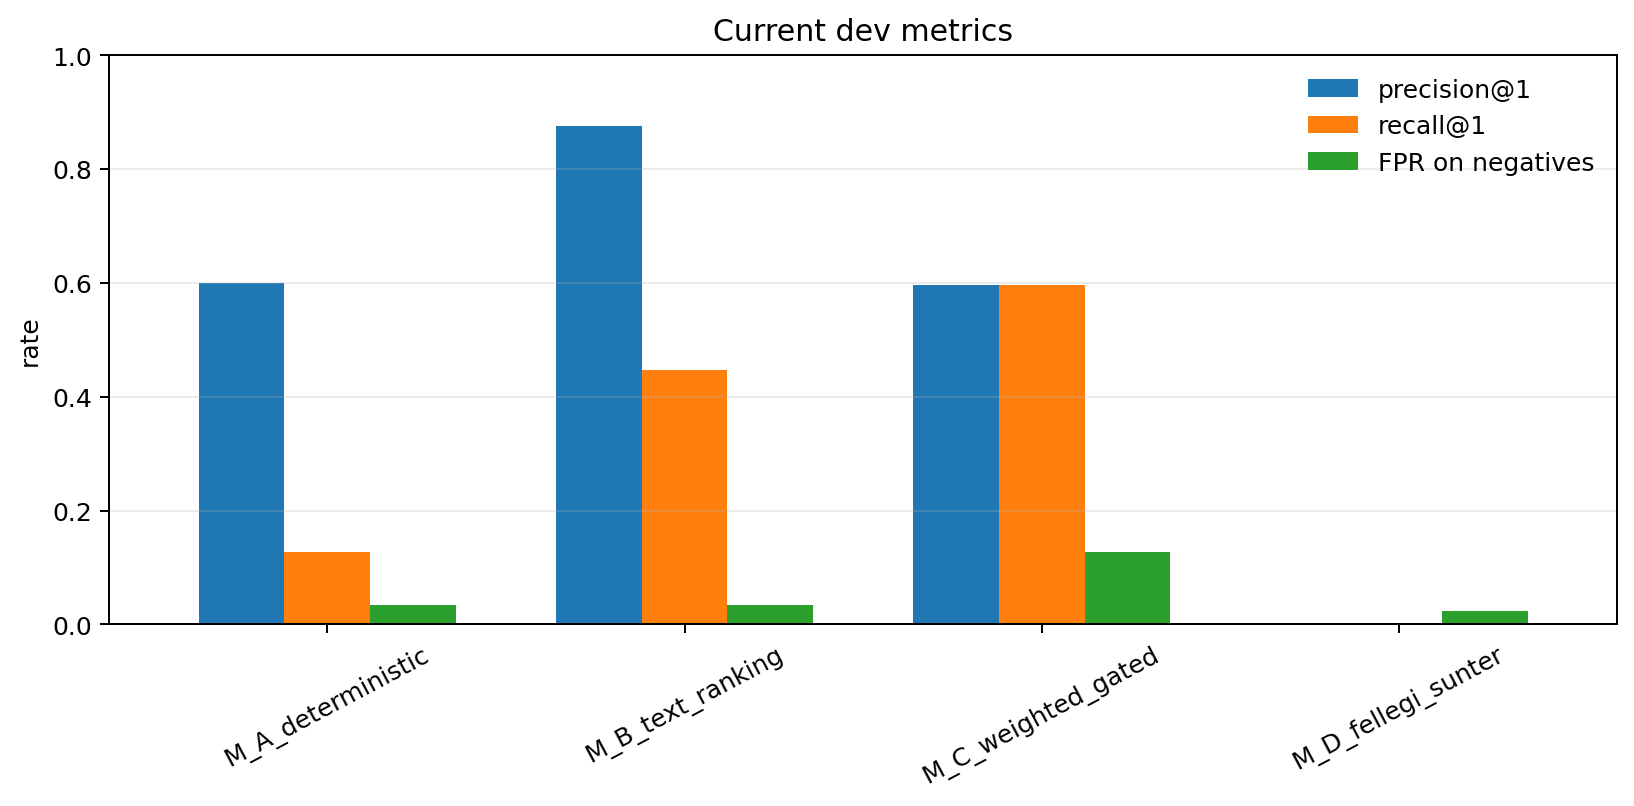
\includegraphics[width=0.92\textwidth]{figures/benchmark_v3_dev_method_metrics.png}
\caption{Dev split method comparison generated from the current benchmark evaluation JSON.}
\end{figure}

\section{Validation Results}
Validation is the method-selection evidence. The primary comparison is
anchor-level exact-successor performance: each anchor can produce one accepted
successor or abstain.
\[
\text{precision}=\frac{TP}{TP+FP},\quad
\text{recall}=\frac{TP}{TP+FN},\quad
\text{FPR}=\frac{FP}{FP+TN}.
\]
For this project, false-positive control is prioritised because false links
fabricate survival events.

\begin{table}[H]
\centering
\small
\begin{tabularx}{\textwidth}{lrrrrrr}
\toprule
Method & Threshold & Accepted & Precision & Recall & FPR & Coverage \\
\midrule
M\_A\_deterministic & 70.000 & 6 & 0.167 & 0.045 & 0.105 & 0.100 \\
M\_B\_text\_ranking & 70.000 & 5 & 0.800 & 0.182 & 0.000 & 0.083 \\
M\_C\_weighted\_gated & 70.000 & 15 & 0.600 & 0.409 & 0.105 & 0.250 \\
M\_D\_fellegi\_sunter & 65.000 & 1 & 0.000 & 0.000 & 0.026 & 0.017 \\
\bottomrule
\end{tabularx}
\caption{Unweighted validation metrics on all labelled current benchmark frames.}
\end{table}

\begin{figure}[H]
\centering
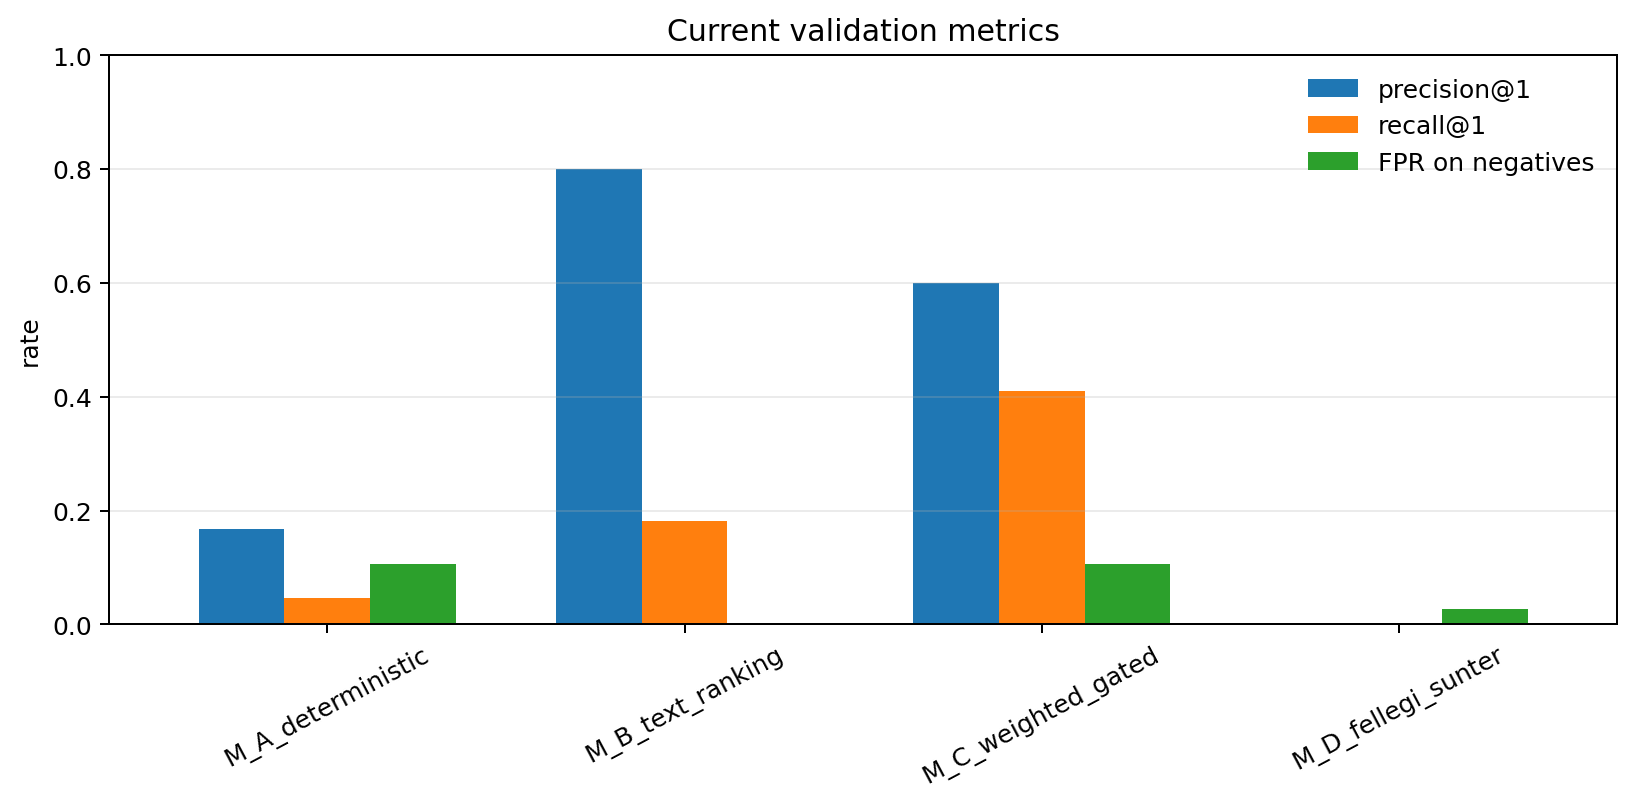
\includegraphics[width=0.92\textwidth]{figures/benchmark_v3_validation_method_metrics.png}
\caption{Validation split method comparison generated from the current benchmark evaluation JSON.}
\end{figure}

\section{Quality Evidence And Interpretation}
The validation result supports a conservative linkage claim. \code{M\_B} has
only 5 accepted validation links, so its precision
estimate is necessarily sample-sensitive; one changed decision would move the
number materially. However, the direction of the evidence is coherent:
\code{M\_B} gives the best validation precision and the lowest false-positive
rate among useful methods, while \code{M\_C} shows the expected precision-recall
trade-off.

The pair-level ROC and precision-recall curves should be read as score-ranking
diagnostics, not as the final operating decision. The final pipeline decision is
anchor-level: choose one successor or abstain. The ROC curve is stepped rather
than smooth because the validation benchmark contains a finite number of
labelled pairs and many tied or near-tied scores.

\section{Modeling Tables}
The modeling-ready tables include strict, primary, broad, and non-match target
columns, plus observable features. They now include the Fellegi--Sunter columns
\code{fs\_match\_weight} and \code{fs\_match\_probability}, so modeling and
evaluation use the same feature state.

\begin{figure}[H]
\centering
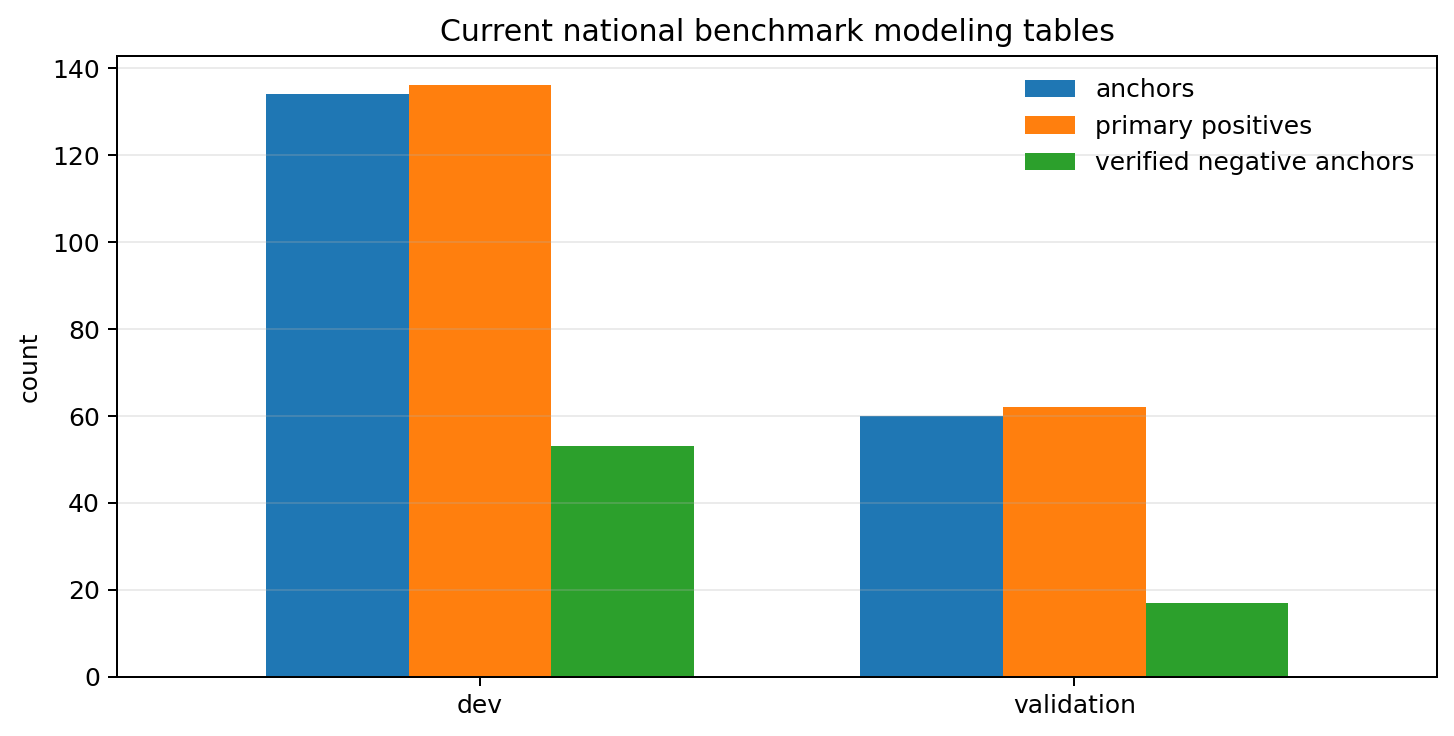
\includegraphics[width=0.86\textwidth]{figures/benchmark_v3_modeling_counts.png}
\caption{Current benchmark modeling table sizes and label support.}
\end{figure}

\section{Survival Results}
The survival dataset uses the main accepted links as events and all other
episodes as right-censored observations at the study cutoff. The main variant
contains 544 events and
3,256 censored observations. Segment
event rates are 0.132
for CPV-32, 0.204
for CPV-35, 0.117
for CPV-48, and 0.143
for CPV-72. CPV-35 has the highest observed successor rate in the main arm.

Sensitivity checks show that absolute event rates depend strongly on the
linkage rule: 296 events under
\code{M\_B @ 0.80}, 544 under
\code{M\_B @ 0.70}, 853 under
\code{M\_B @ 0.60}, and 1,332 under
\code{M\_C @ 0.70}. Therefore the survival estimates should be interpreted as
linkage-conditioned descriptive evidence, not as exact renewal probabilities.

\section{Defensible Decision}
The current defensible decision is to keep \code{M\_B\_text\_ranking @ 0.70}
as the primary observable-successor method and use the stricter, looser,
weighted-gated, and expiry-aware variants as sensitivity analyses. This is a
precision-first design. Low recall is acceptable only because the report frames
the event rate as a lower-bound proxy for visible reprocurement activity:
\[
\text{observed successor rate} \leq \text{true renewal/reprocurement rate}.
\]
If future manual review shows weaker precision, the claim should be narrowed
further rather than forcing a more complex model.

\section{Limitations And Robustness}
\begin{itemize}
\item BOAMP does not consistently encode legal renewal status; accepted links are
observable successor procurements, not legal renewal proof.
\item The current benchmark labels are protocol-generated development evidence with
double-pass validation, not independent human ground truth.
\item Validation is small: 22
positive validation anchors and 5 accepted
\code{M\_B} validation links. The selected threshold should not be over-tuned.
\item Buyer standardisation is improved but remains an important risk area. The
legal-form audit is retained to catch name-only and cross-legal-form cases.
\item Missing duration and expiry fields are not imputed. This avoids creating
false timing certainty.
\end{itemize}

\section{Recommended Reporting Position}
The technical report should defend the project as a reproducible measurement
pipeline, not as a black-box prediction system. The strongest statement is:
\begin{quote}
Because legal renewal status is not directly observed in BOAMP, the study
estimates observable successor procurements. Candidate generation restricts
comparison to the same buyer and a plausible future interval; the selected
method then accepts only the strongest textually similar candidate above a fixed
threshold. This prioritises precision over recall, which is appropriate because
false positive links would create artificial survival events.
\end{quote}

\section{Current Source Files}
\begin{itemize}
\item \pathcode{data/processed/boamp\_v2/linkage\_evaluation\_summary\_v3\_dev\_primary.json}
\item \pathcode{data/processed/boamp\_v2/linkage\_evaluation\_summary\_v3\_validation\_primary.json}
\item \pathcode{data/processed/boamp\_v2/benchmark\_v3/modeling/benchmark\_v3\_modeling\_summary.json}
\item \pathcode{data/processed/boamp\_v2/benchmark\_v3/benchmark\_v3\_manifest.json}
\item \pathcode{data/processed/boamp\_v2/survival\_dataset\_summary.json}
\item \pathcode{data/processed/boamp\_v2/linkage\_candidates\_summary.json}
\end{itemize}

\end{document}
